\documentclass[letterpaper]{article}
\usepackage[utf8]{inputenc}
\usepackage[parfill]{parskip}    % Activate to begin paragraphs with an empty line rather than an indent
\usepackage{graphicx}
\usepackage{amssymb}
\usepackage{amsmath}
\usepackage{amsthm}
\usepackage{mathtools}
\usepackage{mathrsfs}

\usepackage{afterpage}

\usepackage{algorithm}
\usepackage{algpseudocode}

\usepackage{verse}

\newtheorem{theorem}{Theorem}[section]
\newtheorem{corollary}{Corollary}[theorem]
\newtheorem{lemma}[theorem]{Lemma}

\theoremstyle{remark}
\newtheorem*{remark}{Remark}

\usepackage{epstopdf}
\usepackage{circuitikz}
\usepackage[separate-uncertainty = true,multi-part-units=single]{siunitx}
\usepackage{booktabs}
\usepackage{enumitem}
\usepackage[toc,page]{appendix}
\usepackage{color}
\usepackage{pgfplots}
\usepackage{pgfplotstable}
\usepackage{caption}
\usepackage{subcaption}
\usepackage{url}
\usepackage{multirow}
\usepackage{makecell}
\usepackage[round]{natbib}   % omit 'round' option if you prefer square brackets
\usepackage{titling}
\usepackage{siunitx}
\usepackage{physics}

\usepackage{setspace}
% \doublespacing
\usepackage{float}


\pgfplotsset{compat=1.14}

%  Special math symbols
%       floor, ceiling, angled brackets
%-----------------------------------------------------------------------
\newcommand{\floor}[1]{\left\lfloor #1\right\rfloor}
\newcommand{\ceil}[1]{\left\lceil #1\right\rceil}
\newcommand{\etal}{\textit{et al.}}
\newcommand{\RE}{\mathbb{R}}        % real space
\newcommand{\ZZ}{\mathbb{Z}}        % integers
\newcommand{\NN}{\mathbb{N}}        % natural numbers
\newcommand{\eps}{{\varepsilon}}    % prettier epsilon
%-----------------------------------------------------------------------
%  Tighter lists
%-----------------------------------------------------------------------
\newenvironment{itemize*}% Tighter itemized list
  {\begin{itemize}%
    \setlength{\itemsep}{-0.5ex}%
    \setlength{\parsep}{0pt}}%
  {\end{itemize}}
\newenvironment{description*}% Tighter description list
  {\begin{description}%
    \setlength{\itemsep}{-0.5ex}%
    \setlength{\parsep}{0pt}}%
  {\end{description}}
\newenvironment{enumerate*}% Tighter enumerated list
  {\begin{enumerate}%
    \setlength{\itemsep}{-0.5ex}%
    \setlength{\parsep}{0pt}}%
  {\end{enumerate}}
%-----------------------------------------------------------------------
% Typing shortcuts
%-----------------------------------------------------------------------
\newcommand{\X}{\mathbb{X}}
\newcommand{\SG}{\mathbf{S}}
\newcommand{\GE}{\mathcal{G}}
\newcommand{\ST}{\,:\,}
\renewcommand{\tilde}[1]{\widetilde{#1}}
\newcommand{\diam}{\mathrm{diam}}
\newcommand{\sq}{\square}
\newcommand{\half}[1]{\frac{#1}{2}}
\newcommand{\inv}[1]{\frac{1}{#1}}
\newcommand{\alg}{\textsf{SplitReduce}}
\newcommand{\sz}[1]{\sigma_{#1}}
\newcommand{\LL}{\mathcal{L}}
\newcommand{\softOmega}{\widetilde{\Omega}} 
\newcommand{\softO}{\widetilde{O}}
\newcommand{\OO}{O^*}  %or \widetilde{O}?

\newcommand{\Null}[1]{\text{Null}(#1)}


\newcommand{\dx}{\mathrm{d}x}
\newcommand{\dy}{\mathrm{d}y}
\newcommand{\dz}{\mathrm{d}z}
\newcommand{\dt}{\mathrm{d}t}
\newcommand{\du}{\mathrm{d}u}
\newcommand{\dtheta}{\mathrm{d}\theta}
\newcommand{\dq}{\mathrm{d}q}
\newcommand{\diff}{\mathrm{d}}
\newcommand{\dV}{\mathrm{d}V}
\newcommand{\dL}{\mathrm{d}L}
\newcommand{\dA}{\mathrm{d}A}
\newcommand{\dH}{\mathrm{d}H}
\newcommand{\df}{\mathrm{d}f}
\newcommand{\dg}{\mathrm{d}g}
\newcommand{\dr}{\mathrm{d}r}
\newcommand{\dw}{\mathrm{d}w}
\newcommand{\dI}{\mathrm{d}I}

\newcommand*\len[1]{\overline{#1}}


\newcommand\note[1]{\marginpar{\textcolor{red}{#1}}}
\newcommand*{\tageq}{\refstepcounter{equation}\tag{\theequation}}

\newcommand*{\equals}{=}

\usepackage{fancyhdr}

\pgfplotscreateplotcyclelist{grayscale}{
    thick,white!10!black,mark=x,mark options=solid, dashed\\%
    thick,white!20!black,mark=o,mark options=solid\\%
}

\newcommand{\mat}[1]{\ensuremath{\begin{bmatrix}#1\end{bmatrix}}}
\newcommand{\cat}[1]{\ensuremath{\begin{vmatrix}#1\end{vmatrix}}}
\newcommand{\eqn}[1]{\begin{alignat*}{2}#1\end{alignat*}}
\newcommand{\p}[2]{\frac{\partial #1}{\partial #2}}
\newcommand*{\thus}{&\implies\quad&}

\newcommand{\answer}[1]{\framebox{$\displaystyle #1 $}}

\newcommand{\shrug}[1][]{%
\begin{tikzpicture}[baseline,x=0.8\ht\strutbox,y=0.8\ht\strutbox,line width=0.125ex,#1]
\def\arm{(-2.5,0.95) to (-2,0.95) (-1.9,1) to (-1.5,0) (-1.35,0) to (-0.8,0)};
\draw \arm;
\draw[xscale=-1] \arm;
\def\headpart{(0.6,0) arc[start angle=-40, end angle=40,x radius=0.6,y radius=0.8]};
\draw \headpart;
\draw[xscale=-1] \headpart;
\def\eye{(-0.075,0.15) .. controls (0.02,0) .. (0.075,-0.15)};
\draw[shift={(-0.3,0.8)}] \eye;
\draw[shift={(0,0.85)}] \eye;
% draw mouth
\draw (-0.1,0.2) to [out=15,in=-100] (0.4,0.95); 
\end{tikzpicture}}


\pagestyle{fancy}
\fancyhf{}
\rhead{Rahul Arya}
\lhead{EE 16B}
\cfoot{\thepage}

\title{Lecture 20 - Notes}
\author{Rahul Arya}
\date{April 2019}
\begin{document}

\maketitle

\section{Overview}
Last lecture, we considered the singular value decomposition (or SVD) of a matrix, and looked at some of its properties. Now, we will construct a proof of its existence, and explore another of its interpretations. In doing so, we will demonstrate how the SVD of a matrix arises quite naturally from control theory, by considering the problem of \emph{planning} the control of a system.

\section{Planning}
Recall from our understanding of control that any $n$-dimensional discrete-time system with state equation
\[
    \vec{x}[i + 1] = A\vec{x}[i] + B\vec{u}[i]
\]
can be controlled to reach any desired state from any other in at most $n$ time steps if and only if the controllability matrix
\[
    \mathscr{C} = \mat{B & AB & A^2B & \cdots & A^{n-1}B}
\]
is of full row rank. We will only consider the controllable case from now on.

For simplicity, let's consider the case of scalar control only, so $B$ is in fact a column vector. Then, we know that, starting at an initial state $\vec{x}[0] = \vec{0}$, we can reach any target state $\vec{x}^*$ in $n$ time steps by applying the control
\[
    \vec{u} = \mat{u[n - 1] \\ u[n - 2] \\ \vdots \\ u[0]}
\]
chosen such that
\[
    \vec{x}^* = \mat{B & AB & A^2B & \cdots & A^{n-1}B}\mat{u[n - 1] \\ u[n - 2] \\ \vdots \\ u[0]} = \mathscr{C}\vec{u}.
\]

In the case of scalar control, $\mathscr{C}$ is an $n\times n$ matrix (of full rank, by our assumption of controllability) and so is invertible. Thus, we can uniquely choose our control inputs to be
\[
    \vec{u} = \mathscr{C}^{-1}\vec{x}^*.
\]

However, what if we didn't want to arrive at the state $\vec{x}^*$ after $n$ time steps, but only need to be there after some longer duration $t > n$? Clearly, there are many ways to do so. In particular, notice that for the first $t - n$ steps, we can apply \emph{any} controls we want, since the final $n$ steps will always be sufficient to bring us to $\vec{x}^*$.

So are we done? Not quite. Imagine the linear system of our robot car from lab, and consider the problem of bringing it to a particular state (i.e. assigning particular values to the wheel velocities) at a certain time. One way (that is perhaps the most natural) would be to apply a steady input to gradually ramp up the wheel velocities, so we reach the target state at the desired time. Another way, however, could be to apply large random inputs, accelerating and decelerating each wheel, until just before the target time $t$, at which point we would apply large controls to set the wheel velocities to their desired values. Clearly, though both approaches accomplish the same goal, the former is more ``natural'' than the latter.

More generally, in the case of arbitrary controllable linear systems, we will aim to choose a series of scalar inputs $\vec{u}$ that reach the target state while minimizing a cost function, which expressed how ``unnatural'' our inputs are. 

An obvious choice for this cost function would be the norm $\norm{\vec{u}}$ of the inputs. In our earlier example of the robot car, it should be clear that the first case of applying steady inputs has a smaller norm than the large, randomly varying inputs of the second case, suggesting that this definition of the cost function is in accordance with our intuition. We will aim to compute the control input that reaches a target value while minimizing this quantity, known as the \emph{minimum energy control}.

\section{Minimum Energy Control}
In the previous section, we focused on controllable systems with scalar inputs, where $\mathscr{C}$ was of full rank. Now, we will consider the more general problem of arbitrary $n$-dimensional systems with scalar inputs, with an initial state $\vec{x}[0] = \vec{0}$. We will denote
\[
    \mathscr{C}_t = \mat{B & AB & A^2B & \cdots & A^{t-1}B}
\]
where $A$ and $B$ are the matrices in the state transition equation.

By expanding out the state transition matrix, it is clear that we wish to choose the $t$-dimensional input vector $\vec{u}$ such that
\[
    \vec{x}[t] = \mathscr{C}_t\vec{u} = \vec{x}^*.
\]
We will assume that $\vec{x}^*$ lies in the column space of $\mathscr{C}_t$, as otherwise the problem is clearly unsolvable since the target state can never be reached. But since $\mathscr{C}$ may have a null space, it is possible for infinitely many solutions $\vec{u}$ to exist, and we wish to pick the solution with minimum norm.

Let's try to make sense of this problem by drawing a picture. Let $\vec{u}_0$ be a particular solution to the above equation (that is not necessary of minimum norm), and recall that the null space of $\mathscr{C}_t$ is a subspace of $t$-dimensional space. Furthermore, observe that for any vector $\vec{a} \in \Null{\mathscr{C}_t}$, $\vec{u}_0 + \vec{a}$ is a solution to our equation, since
\[
    \mathscr{C}_t(\vec{u}_0 + \vec{a}) = \mathscr{C}_t\vec{u}_0 + \mathscr{C}\vec{a} = \mathscr{C}_t\vec{u}_0 = \vec{x}^*.
\]
Although we will not prove it here, it is extremely straightforward to see that any possible solution $\vec{u}$ where $\mathscr{C}_t\vec{u} = \vec{x}^*$ can be written in the form $\vec{u}_0 + \vec{a}$ for some $\vec{a} \in \Null{\mathscr{C}_t}$.

Thus, we can plot the space of possible $\vec{u}$ by first plotting all vectors in $\Null{\mathscr{C}_t}$, and then translating them by $\vec{u}_0$, as shown\footnote{Note that the figure represents $\mathscr{C}_t$ as $\mathcal{C}_t$ because I can't figure out how to import \LaTeX \, packages into my drawing software}:
\begin{center}
    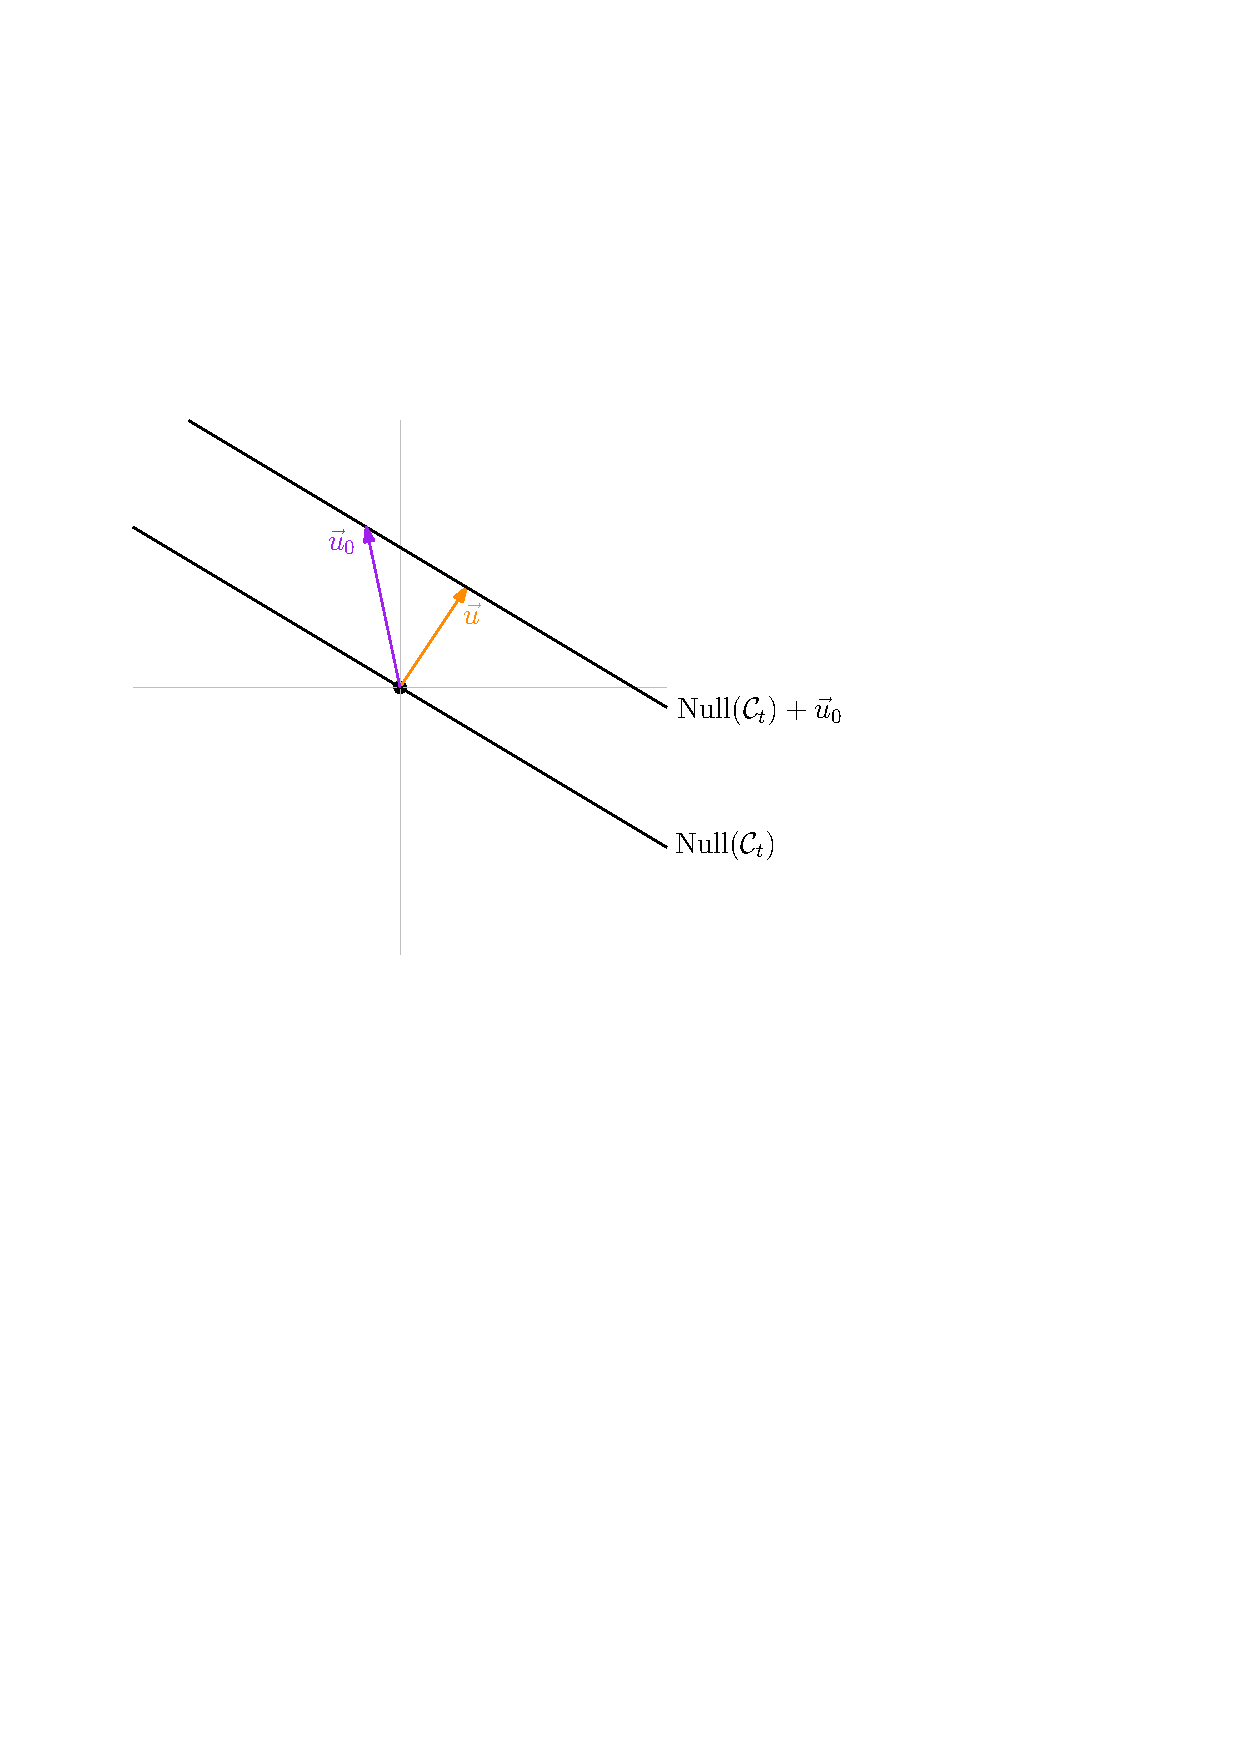
\includegraphics[scale=0.7]{lecture_20/subspaces.pdf}
\end{center}
Intuitively, from the figure, it seems clear that the control input $\vec{u}$ with minimum norm should be one that is entirely orthogonal to $\Null{\mathscr{C}_t}$. This would seem to be analogous to what we saw when studying least squares, where again we were interested in choosing a point on a subspace such that the error vector was orthogonal to said subspace.

Let's try to prove this rigorously. Imagine that we had some orthonormal basis
\[
    \vec{v}_1, \vec{v}_2, \ldots, \vec{v}_t
\]
of our $t$-dimensional space of inputs, such that the first $n$ $\vec{v}_1, \ldots, \vec{v}_n$ form a basis for those vectors orthogonal to $\Null{\mathscr{C}_t}$, and the remaining $t - n$ vectors $\vec{v}_{n+1}, \ldots, \vec{v}_t$ form a basis for $\Null{\mathscr{C}_t}$. We will worry about constructing this basis later - for now, let's just assume that it exists.

Consider our $\vec{u}_0$ expressed in this basis, as follows:
\[
    \vec{u}_0 = \alpha_1\vec{v}_1 + \alpha_2\vec{v}_2 + \ldots + \alpha_n\vec{v}_n.
\]
Observe that the norm of $\vec{u}_0$ is
\eqn{
    && \norm{\vec{u}_0} &= \sqrt{\vec{u}_0 \cdot \vec{u}_0} \\
    &&&= \sqrt{\alpha_1^2 + \alpha_2^2 + \ldots + \alpha_n^2},
}
since the $\vec{v}_i$ are orthonormal, so $\vec{v}_i \cdot \vec{v}_j$ is $1$ if $i = j$ and $0$ otherwise.

Now, observe that in this basis, any $\vec{a} \in \Null{\mathscr{C}_t}$ can be represented as
\[
    \vec{a} = \beta_{t+1}\vec{v}_{t+1} + \beta_{t+2}\vec{v}_{t+2} + \ldots + \beta_n\vec{v}_n,
\]
since (by definition) it has components only in the the null space of $\mathscr{C}_t$. Thus, we can write any solution $\vec{u} = \vec{u}_0 + \vec{a}$ as
\[
    \vec{u} = \vec{u}_0 + \vec{a} = \alpha_1\vec{v}_1 + \alpha_2\vec{v}_2 + \ldots + \alpha_n\vec{v}_n + (\alpha_{n+1}-\beta_{n+1})\vec{v}_{n + 1} + \ldots + (\alpha_t - \beta_t)\vec{v}_t.
\]
In a similar manner to what we did before, we see immediately that the norm of this expression is
\[
    \norm{\vec{u}} = \sqrt{\alpha_1^2 + \alpha_2^2 + \ldots + \alpha_n^2 + (\alpha_{n+1}-\beta_{n+1})^2 + \ldots + (\alpha_t - \beta_t)^2}.
\]
To minimize the norm of $\vec{u}$, therefore, it is clear that we should set the $\beta_i = \alpha_i$ for all valid $i > n$. Therefore, our minimum energy control must be
\eqn{
    && \vec{u} &= \vec{u}_0 + \vec{a} \\
    &&&= \alpha_1\vec{v}_1 + \alpha_2\vec{v}_2 + \ldots + \alpha_n\vec{v}_n + (\alpha_{n+1}-\beta_{n+1})\vec{v}_{n + 1} + \ldots + (\alpha_t - \beta_t)\vec{v}_t \\
    &&&= \alpha_1\vec{v}_1 + \alpha_2\vec{v}_2 + \ldots + \alpha_n\vec{v}_n + (\alpha_{n+1}-\alpha_{n+1})\vec{v}_{n + 1} + \ldots + (\alpha_t - \alpha_)\vec{v}_t \\
    &&&= \alpha_1\vec{v}_1 + \alpha_2\vec{v}_2 + \ldots + \alpha_n\vec{v}_n.
}
Observe that this solution is entirely orthogonal to $\Null{\mathscr{C}_t}$, as we had expected. All that remains now is to demonstrate the existence of the $\vec{v}_i$.

\section{Constructing an Orthonormal Basis}
In truth, this task is rather simple. From Gaussian elimination, we know how to compute a basis of $\Null{\mathscr{C}_t}$, which we can orthonormalize using Gram-Schmidt to produce the $\vec{v}_{n+1}, \ldots, \vec{v}_n$. We can then extend this basis again using Gram-Schmidt to span all of $t$-dimensional space, to produce the $\vec{v}_1, \ldots, \vec{v}_t$, demonstrating the existence of our desired basis. Although this description is not fully precise, it is very straightforward to make it rigorous and solve the problem of minimum energy control.

However, we will choose to attack this problem from a different direction, which is not entirely unreasonable and will prove useful in our later derivation of the SVD. By definition, the $\vec{v}_i$ are an orthonormal basis of $t$-dimensional space. But recall from last lecture that, by the real spectral theorem, the eigenvectors of a real symmetric matrix can also form such an orthonormal basis. Wouldn't it be interesting if some symmetric matrix $Q$ had exactly these eigenvectors $\vec{v}_1, \ldots, \vec{v}_t$?

Furthermore, observe that $\vec{v}_{n+1}, \ldots, \vec{v}_t$ are in fact all eigenvectors of $\mathscr{C}_t$ as well?! Why? Well, they're members of $\Null{\mathscr{C}_t}$, which is simply the eigenspace of $\mathscr{C}_t$ corresponding to $\lambda = 0$. It is natural to make the additional conjecture that, not only will these $\vec{v}_{n+1}, \ldots, \vec{v}_t$ be eigenvectors of our $Q$, but they will in fact be eigenvectors with eigenvalue $0$, so they will lie in its null space.

How do we generate such a symmetric matrix $Q$? Since it has the same null space as $\mathscr{C}_t$, perhaps we could try writing it in the form
\[
    Q = D\mathscr{C}_t,
\]
where $D$ is some unknown matrix of full column rank, so $Q$ and $\mathscr{C}_t$ clearly have the same eigenspace. Now, as $Q$ is symmetric, we can take transposes to obtain
\[
    Q^T = \mathscr{C}_t^TD^T \implies D\mathscr{C}_t = \mathscr{C}_t^TD^T.
\]
Looking at the latter equality, a natural conjecture would be $D = \mathscr{C}_t^T$, so $Q = \mathscr{C}_t^T\mathscr{C}_t$. Let's see if this works out.

It is obvious that $\Null{\mathscr{C}_t} \subseteq \Null{Q}$. Let's try to prove the opposite relation, in order to show equality. Specifically, for any $\vec{v} \in \Null{Q}$, we'd like to show that $\vec{v} \in \Null{\mathscr{C}_t}$. Well, for any given such $\vec{v}$, by definition it is true that
\[
    Q\vec{v} = \vec{0} \implies \mathscr{C}_t^T\mathscr{C}_t\vec{v} = \vec{0}.
\]
We'd like to show that $\mathscr{C}_t\vec{v} = \vec{0}$, which is equivalent to writing $\norm{\mathscr{C}_t\vec{v}} = 0$. By the definition of the norm of a real vector, we'd like to show that
\[
    (\mathscr{C}_t\vec{v})^T(\mathscr{C}_t\vec{v}) = \vec{v}^T\mathscr{C}_t^T\mathscr{C}_t\vec{v} = 0.
\]
But wait! This is basically what we had in the definition of $\vec{v}$, just pre-multiplied by $\vec{v}^T$. Putting everything together into a proof, we have
\eqn{
    && \vec{v} &\in \Null{Q} \\
    \thus Q\vec{v} &= \vec{0} \\
    \thus \mathscr{C}_t^T\mathscr{C}_t\vec{v} &= \vec{0} \\
    \thus \vec{v}^T\mathscr{C}_t^T\mathscr{C}_t\vec{v} &= 0 \\
    \thus \norm{\mathscr{C}_t\vec{v}} &= 0 \\
    \thus \mathscr{C}_t\vec{v} &= \vec{0} \\
    \thus \vec{v} &\in \Null{\mathscr{C}_t},
}
so $\Null{Q} \subseteq \Null{\mathscr{C}_t}$, as we desired. Since we've proven this inequality in both directions, we have $\Null{Q} = \Null{\mathscr{C}_t}$, as we had hoped.

Thus, we can produce an orthonormal basis of the eigenspace corresponding to $\lambda = 0$ of $Q$ that provides us with the $\vec{v}_{n+1}, \ldots, \vec{v}_t$ that we wanted.

Considering the remaining eigenvectors of $Q$ for $\lambda \ne 0$, it is clear (by the real spectral theorem) that they can be divided into mutually orthogonal eigenspaces that will all be orthogonal to $\Null{Q}$, so we can choose $n$ of them to form our $\vec{v}_1, \ldots, \vec{v}_n$, completing our construction of the $\{ \vec{v}_i \}$.

\section{Singular Values}
Now that we know how to construct this $Q$, and have demonstrated that its eigenvectors are exactly the $\vec{v}_1, \ldots, \vec{v}_t$ that we had wanted, it is natural to speculate on the eigenvalues of each of these eigenvectors. We know that the eigenvalues of $\vec{v}_{n + 1}, \ldots, \vec{v}_t$ are all $0$, since they lie in the null space of $Q$. But what about the first $n$ eigenvectors? Let's try to work this out algebraically. 

By the definition of eigenvectors, we can perform manipulations very similar to what we did earlier involving nullspaces, to see that
\eqn{
    && Q \vec{v}_i &= \lambda_i \vec{v}_i \\
    \thus \mathscr{C}_t^T\mathscr{C}_t &= \lambda_i\vec{v}_i \\
    \thus \vec{v}_i^T\mathscr{C}_t^T\mathscr{C}_t &= \lambda_i \vec{v}_i^T \\
    \thus \vec{v}_i^T\mathscr{C}_t^T\mathscr{C}_t\vec{v}_i &= \lambda_i \vec{v}_i^T\vec{v}_i \\
    \thus \norm{\mathscr{C}_t\vec{v}_i}^2 &= \lambda_i \norm{\vec{v}_i}^2 \\
    \thus \lambda_i &= \frac{\norm{\mathscr{C}_t\vec{v}_i}^2}{\norm{\vec{v}_i}^2} \\ 
    &&&= \norm{\mathscr{C}_t\vec{v}_i}^2.
}
In particular, notice that $\lambda_i \ge 0$. For $i > n$, we already knew that $\lambda_i = 0$. But for $i \le n$, since $\vec{v}_i \not\in \Null{\mathscr{C}_t}$, $\lambda_i \ne 0$, so $\lambda_i > 0$.

This sounds interesting. Without loss of generality, we can order our $\vec{v}_i$ such that
\[
    \lambda_1 \ge \lambda_2 \ge \ldots \ge \lambda_n > \lambda_{n + 1} = \lambda_{n + 2} = \ldots = \lambda_t = 0,
\]
and place them as columns of the eigenvector matrix
\[
    V = \mat{| & & | \\ \vec{v}_1 & \cdots & \vec{v}_t \\ | & & |}.
\]
We can then write the eigendecomposition of $Q$ as
\[
    Q = V\Lambda V^{-1} = V\mat{\lambda_1 & 0 & \ldots &  0 \\ 0 & \lambda_2 & \ldots & 0 \\ \vdots & \vdots & \ddots & \vdots \\ 0 & 0 & \ldots & \lambda_t}V^T.
\]
Since all the $\lambda_i \ge 0$, we can choose
\[
    \sigma_1 \ge \sigma_2 \ge \ldots \ge \sigma_n > \sigma_{n + 1} = \sigma_{n + 2} = \ldots = \sigma_t = 0
\]
where $\lambda_i = \sigma_i^2$ for all $i$. Recall that $\lambda_i = \norm{\mathscr{C}_t\vec{v}_i}^2$, so $\sigma_i = \norm{\mathscr{C}_t\vec{v}_i}$. These $\sigma_i$ are known as the \emph{singular values} of $\mathscr{C}_t$, and will prove important in the next section.

\section{Constructing Another Orthonormal Basis}
At this point, we will make what may appear to be an unintuitive step. Up until now, the argument has followed a fairly straightforward path, with the choice of each new step intuitively justified (at least to some extent) from the previous. Now, however, we will make a conjecture that may not seem particularly reasonable. It could have been obtained through random manipulations, out of sheer curiosity, or perhaps by observing an interesting property of a numerical example.

Regardless, here it is: just as the $\vec{v}_i$ were mutually orthogonal, we conjecture that the set of $\mathscr{C}_t\vec{v}_i$ is mutually orthogonal too. Let's see why. For any valid choice of $i \ne j$, we see that
\eqn{
    && (\mathscr{C}_t\vec{v}_i) \cdot (\mathscr{C}_t\vec{v}_j) &= \vec{v}_j\mathscr{C}_t^T\mathscr{C}_t\vec{v}_i \\
    &&&= \sigma_i^2 \vec{v}_j^T\vec{v}_i \\
    &&&= 0,
}
since $\vec{v}_i$ and $\vec{v}_j$ are orthogonal. Thus, our conjecture is true!

If the $\mathscr{C}_t\vec{v}_i$ are orthogonal, it'd be reasonable to try and use them to create an orthonormal basis of the column space of $\mathscr{C}_t$. Recall that $\mathscr{C}_t\vec{v}_i = \vec{0}$ for all $i > n$ as those $\vec{v}_i \in \Null{\mathscr{C}_t}$, so those vectors will not be contributing to our basis. 

But we still have $n$ nonzero mutually orthogonal vectors corresponding to $i \le n$, and the column space of $\mathscr{C}_t$ is $n$ dimensional, so we're still OK! To make each of these vectors of unit length, we should scale them down by their length $\norm{\mathscr{C}_t\vec{v}_i} = \sigma_i$, to obtain the orthonormal basis $\vec{w}_1, \vec{w}_2, \ldots, \vec{w}_n$, where we define
\[
    \vec{w}_i = \frac{\mathscr{C}_t\vec{v}_i}{\sigma_i}
\]
for all valid $i \le n$. Rearranging, we get
\[
    \mathscr{C}_t\vec{v}_i = \sigma_i\vec{w}_i.
\]
Horizontally stacking this result for all $i \le n$m, we find that
\[
    \mathscr{C}_t \mat{| & & | \\ \vec{v}_1 & \cdots & \vec{v}_n \\ | & & |} = \mat{| & & | \\ \vec{w}_1 & \cdots & \vec{w}_n \\ | & & |} \mat{\sigma_1 & 0 & \ldots &  0 \\ 0 & \sigma_2 & \ldots & 0 \\ \vdots & \vdots & \ddots & \vdots \\ 0 & 0 & \ldots & \sigma_n}.
\]
This is probably beginning to look very familiar, since it's practically the singular value decomposition of $\mathscr{C}_t$! What's missing? Well, recall that each of the $\vec{v}_i$ was $t$ dimensional, but we only use $n$ of them here, so the matrix stacking them horizontally is not square! To fix this, we can simply ``pad'' that matrix with the remaining $\vec{v}_i$ for $i > n$, and introduce additional zero columns to the diagonal matrix of the $\sigma_i$, to obtain
\[
    \mathscr{C}_t \mat{| & & | \\ \vec{v}_1 & \cdots & \vec{v}_t \\ | & & |}^T = \mat{| & & | \\ \vec{w}_1 & \cdots & \vec{w}_n \\ | & & |} \mat{\sigma_1 & 0 & \ldots & 0 & 0 & \ldots & 0 \\ 0 & \sigma_2 & \ldots & 0 & 0 & \ldots & 0 \\ \vdots & \vdots & \ddots & \vdots & \vdots & \ddots & \vdots \\ 0 & 0 & \ldots & \sigma_n & 0 & \ldots & 0},
\]
Now, since $V$ is a square orthogonal matrix, $V^{-1} = V^T$, so we can rearrange to obtain
\[
    \mathscr{C}_t = \mat{| & & | \\ \vec{w}_1 & \cdots & \vec{w}_n \\ | & & |} \mat{\sigma_1 & 0 & \ldots & 0 & 0 & \ldots & 0 \\ 0 & \sigma_2 & \ldots & 0 & 0 & \ldots & 0 \\ \vdots & \vdots & \ddots & \vdots & \vdots & \ddots & \vdots \\ 0 & 0 & \ldots & \sigma_n & 0 & \ldots & 0}\mat{| & & | \\ \vec{v}_1 & \cdots & \vec{v}_t \\ | & & |}^T = W\Sigma V^T,
\]
defining $U$ and $\Sigma$ to be the horizontally stacked $\vec{w}_i$ and the diagonal matrix of the $\sigma_i$ respectively.

\section{Applications to Planning}
Finally, we have obtained the singular value decomposition of $\mathscr{C}_t$. Notice that we have found a new way to interpret it - the columns of $V$ formed a $t$-dimensional orthonormal basis of the domain of $\mathscr{C}_t$, and the columns of $W$ formed an $n$-dimensional orthonormal basis of its column space.

Moreover, they mapped between each other in a very clean manner, with $\mathscr{C}_t\vec{v}_i = \sigma_i\vec{w}_i$ for $i \ne n$, and $\mathscr{C}_t\vec{v}_i = \vec{0}$ for $i > n$. Let's see how we can use this property of the SVD can help us find the minimum cost control input.

Recall that we showed that our control vector $\vec{u}$ must have components only along $\vec{v}_1, \ldots, \vec{v}_n$, in order to minimize its norm. Thus, for $\mathscr{C}_t\vec{u} = \vec{x}^*$, we can use projections onto these two bases to see that
\eqn{
    && \mathscr{C}_t\vec{u} &= \vec{x}^* \\
    \thus \mathscr{C}_t \left(\sum_{i=1}^n (\vec{u} \cdot \vec{v}_i) \vec{v}_i\right) &= \sum_{i=1}^n (\vec{x}^* \cdot \vec{w}_i)\vec{w}_i \\
    \thus \sum_{i=1}^n (\vec{u} \cdot \vec{v}_i) (\mathscr{C}_t\vec{v}_i) &= \sum_{i=1}^n (\vec{x}^* \cdot \vec{w}_i)\vec{w}_i \\
    \thus \sum_{i=1}^n \sigma_i(\vec{u} \cdot \vec{v}_i) \vec{w}_i &= \sum_{i=1}^n (\vec{x}^* \cdot \vec{w}_i)\vec{w}_i,
}
so
\[
    \sigma_i(\vec{u} \cdot \vec{v}_i) = (\vec{x}^* \cdot \vec{w}_i)\vec{w}_i \implies \vec{u} \cdot \vec{v}_i = \frac{(\vec{x}^* \cdot \vec{w}_i)\vec{w}_i}{\sigma_i}.
\]
for all valid $i \ne n$. Substituting back into our expression for $\vec{u}$, recalling that it does not have any components in $\Null{\mathscr{C}_l}$, we obtain
\[
    \vec{u} = \sum_{i=1}^n \frac{(\vec{x}^* \cdot \vec{w}_i)\vec{w}_i}{\sigma_i} \vec{v}_i,
\]
which is a clean expression for the minimum energy control to reach our desired state in terms of the SVD.

\end{document}
